\section{Обзор}
В разделе рассмотрены технологии программирования 
гетерогенных вычислительных систем, в которых CPU управляет GPGPU,
задача гомологичности и её существующие решения.

\subsection[Технологии программирования гетерогенных систем] {Технологии программирования гетерогенных\\вычислительных систем}
Здесь кратко описаны различные языки программирования систем вида 
CPU и GPGPU, а также их инфраструктура.

\subsubsection{\name{NVIDIA CUDA}}
\name{CUDA} (Compute Unified Device Architecture)~\cite{CUDA} --- 
это платформа параллельных вычислений и программный интерфейс 
для управления видеокартами.
\name{CUDA} является пропиетарной разработкой компании \name{NVIDIA}.
Исходный код на \name{CUDA} транслируется в \name{PTX} ---
псевдо-ассемблерное промежуточное представление, 
которое драйвер видеокарты переводит в бинарный код.
\name{CUDA} предназначена только для работы с GPGPU от \name{NVIDIA}.
%TODO как компилируется ядро? PTX появляется на стадии компиляции или в рантайме?
%TODO типобезопасность?

\subsubsection{\name{OpenCL} и \name{SYCL}}
Разнообразие оборудования и интерфейсов усложняет поддержку
программного обеспечения.
Представителями индустрии была сформирована \name{Khronos Group} с целью
разработки общих открытых стандартов программирования центральных процессоров 
и видеокарт.

Одним из результатов работы группы стал стандарт 
\name{OpenCL}~\cite{OpenCL} --- программный интерфейс для доступа к любому
устройству, которое предоставляет соответствующий драйвер.
Для разработки кода ядра используется диалект
языка \name{C99} с некоторыми ограничениями.
Управление памятью в \name{OpenCL} ручное, программист должен явно указывать,
каким образом и когда передавать данные на требуемое устройство.
Изначально ядро нужно было компилировать во время исполнения, 
то есть каждый раз при запуске программы, даже если само ядро не менялось.
Такой вариант называется онлайн компиляцией, которая необходима для 
обеспечения переносимости.

Позднее появился стандарт \name{SPIR-V}~\cite{SPIR-V}, который описывает 
переносимое промежуточное представление.
\name{SPIR-V} можно перевести в \name{LLVM IR}~\cite{LLVM} и наоборот.
Стало возможным единовременно компилировать весь исходный код с помощью 
инфраструктуры \name{LLVM}.
Cпособ, когда ядро во время стадии компиляции исходного кода переводится в
\name{SPIR-V}, а затем используется \name{LLVM}, 
называется оффлайн компиляцией.

Наличие этих двух стандартов привело к созданию \name{SYCL}~\cite{SYCL}.
Это высокоуровневая абстракция на \name{С++} над \name{OpenCL} с полной
обратной совместимостью.
В отличие от \name{OpenCL}, при использовании \name{SYCL} не нужно 
манипулировать памятью, программист только указывает, какие данные требуются 
для выполнения кода ядра.
На стадии компиляции строится граф управления передачей данных между 
устройствами, что значительно уменьшает вероятность некорректной работы 
с памятью.
Ядро пишется на стандартном \name{C++} в коде исходного приложения 
с некоторыми ограничениями --- нельзя использовать исключения, указатели на
функции и виртуальные функции, но можно применять лямбда-выражения, шаблоны, 
наследование и другие абстракции.
Такой дизайн (рис.~\ref{SYCL_infrastructure}) позволяет компилятору 
использовать систему типов \name{C++} для создания оптимизированного кода.
\begin{figure}
  \centering
  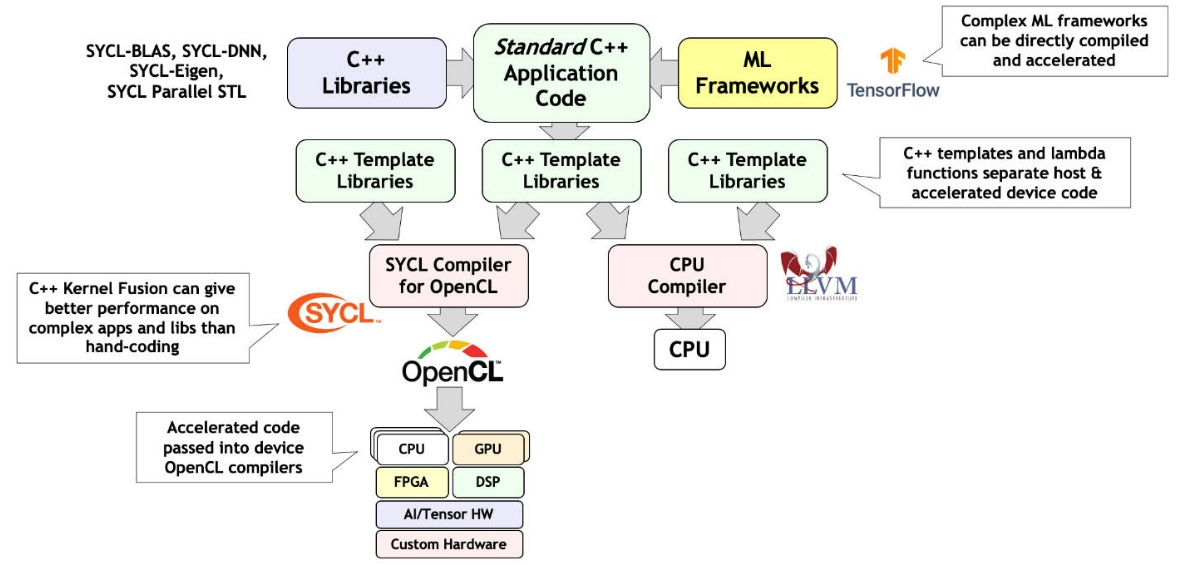
\includegraphics[width=\columnwidth]{sycl.jpg}
  \caption{Инфраструктура приложения с использованием \name{SYCL}}
  \label{SYCL_infrastructure}
\end{figure}

Сейчас есть четыре реализации стандарта \name{SYCL}: 
\name{ComputeCpp}~\cite{ComputeCpp} от Codeplay,
\name{DPC++}~\cite{DPC} от \name{Intel},
\name{hipSYCL}~\cite{hipSYCL},
\name{triSYCL}~\cite{triSYCL} от \name{AMD} и \name{Xilinx}.
Первая реализация распространяется бесплатно в виде разделяемой библиотеки,
а последние являются проектами с открытым исходным кодом.
На данный момент \name{ComputeCpp} является наиболее соответствующей 
стандарту реализацией.
Также идет работа над тем, чтобы переводить код с использованием \name{SYCL} на 
эквивалентный \name{CUDA} код, так как приложения на \name{OpenCL} или
\name{SYCL} для GPGPU от \name{NVIDIA} менее производительны, чем аналогичные 
на \name{CUDA} из-за лимитированной поддержки стандарта \name{OpenCL} на этих 
устройствах со стороны \name{NVIDIA}.

\subsection{Задача гомологичности}
Еще раз про гомологичность, СММ.
\subsubsection{HMMer}
\subsubsection{Cudampf}

В теории, можно посмотреть в userguide HMMer.
